\section{Introduction}

% \textit{Evolution strategies (ESs)} have been widely utilized to solve optimization problems where the true objective function evaluation is computationally-intensive. The use of a population of candidate solutions makes ESs invariant to moderate noise and transformation. To extend the benefit of a potential large population size, one way is to use surrogate model, a substitution of the true objective function built based on the information of previous iterations. A surrogate can be built either as a local approximation or a global approximation to the true objective function \cite{Jin:2002:FAE:2955491.2955686}. It give a more computationally efficient inaccurate estimate of the offsprings' fitness, replacing the expensive true objective function evaluation. The estimate using surrogate model yields insight into potential avoidance of poor step size. 

\textit{Evolution strategies (ESs)} have been widely utilized to solve optimization problems where the true objective function evaluation is computationally-intensive. Various attempts have been made to reducte the cost by extracting the information obtained from points evaluated in previous iterations. Such information yields insights into better mutation and recombination that help generate and select promising offspring. Cummulative step size adaptation (CSA) \cite{Ostermeier:1994:DAS:1326675.1326679} builds an evolution path based on the history step size (mutation) of ESs, the population in the next iteration is generated based on the mutation adpated by the evolution path. 

The history information could be used to construct a surrogate model, referred either as a local approximation or a global approximation to the true objective function \cite{Jin:2002:FAE:2955491.2955686}. There are a range of surrogate models and a survey of the development can be found by Jin \cite{JIN201161} and Loshchilov \cite{ECJ2016_LMCMA}. Those algorithms are usually heuristic by nature and the behaviour of each step is likely not well interpreted. Recent work in surrogate assisted EAs tend to use sophosticated algroithm where surrogates are combined or the model is updated online according to some heustic. Comparision is often made by comparing the performance using the algorithm with and without model assistance where the behaviour of the surrogate is not well simulated. In this context, an approach that could simulate the surrogate would be helpful in understanding the surrogate behaviour, leading to potential modification for surrogate update or parameter-setting. A surrogate that models the objective function with desired precise gains benefit especially for algorithms that requires a large population size for good performance.The computational saving largely lies in the saved evaluations outshine the potential poor step resulted from relative inaccurate estimation of candidate solutions. 


% It give a more computationally efficient inaccurate estimate of the offsprings' fitness, replacing the expensive true objective function evaluation. The estimate using surrogate model yields insight into potential avoidance of poor step size resulted from poor estimation of candidate solution.  A surrogate model can either filter or rank the population generated in each iteration with vanishing cost, acting as a pre-selection of candidate solutions. The effectiveness of using surrogate model largely lies in the model accurancy that the candidate solutions can be effectively filtered or ranked. 

This paper intend to improve the understanding of the impact of population size on surrogate-assisted ESs' by analyzing using simple test functions with strong theoretical basis and established baselines. The paper is organized as follows: In Section 2 we give a brief review of related background, in Section 3 we propose a local surroagte model-assisted $((\mu/\mu,\lambda)+(\mu/\mu,\lambda))$-ES and study its behaviour on sphere functions. Based on the existing knowledge and step behaviour, in Section 4, we then propose a combined step size adaptation mechanism for the this algorithm, analyze the performance using several test functions and compare the result with a surrogate model-assisted (1+1)-ES \cite{DBLP:conf/ppsn/KayhaniA18}. The experimental result is followed by a discuession and future work in Section 5. 


% The effectiveness of surrogate assisted model is that it either effectively filter those undesired candidate solutions (reduce the population size) so that the unnecessary objective function evaluations can be avoided. It is the reduction of the population size by filtering undesired candidate solutions rather than the surrogate mode that saves the computational cost directly \cite{ARASH}.


% By using a similar idea to surrogated model assisted EAs, we do not use a local surrogate model to do the pre-selection in each iteration. Instead, we use it to optimize the candidate solutions obtained in each iteration by fitting a quadratic model in one dimension. By taking the lowest point of the quadratic model as the offspring of this iteration, we hope the fitness of the offspring obtained by the quadratic model would be better compared with the candidate solution directly generated from the parent. For better interpretation, we study the behavior of the proposed surrogate model assisted EAs using simple test functions, allowing comparisons with established basslines. The contributions of this paper are as follows: in Section 2, we give a brief review of related background, in Section 3, we propose a local surrogate model assisted (1+1)-ES, in Section 4, the model is evaluated on quadratic sphere following the same framework proposed by Kayhani and Arnold \cite{ARASH}. 

% \begin{figure*}
% \includegraphics[height=2.6in, width=7in]{matlabcode}
% \caption{MATLAB code for the proposed local surrogate model }
% \end{figure*}





\section{Related Work}

\subsection{Surrogate Model} 
% Def of surrogate model 

Using an approximate model to reduce computational cost can be traced back to 1960s \cite{dunham1963design}. Some successful surrogated models include but are not limitted to Polynomial Regression (PR, response surface methodology) \cite{doi:10.1080/00401706.1966.10490404}, Gaussian Process (GP, Kriging models) \cite{sacks1989}, Artificial neural networks \cite{Smith:1993:NNS:583180}. There are two types of surrogate models, global surrogate model and local surrogate model, . ES using global surrogate model based on Kring was examined by Ratle \cite{Ratle:2001:KSF:966173.966177}. Another ES using global surrogate model based on Artificial neural networks was constructed by Jin \cite{Jin02aframework} which gives an imperial criterion on using the true objective function or the surrogate model to evaluate the offspring. Ulmer et al \cite{Ulmer03evolutionstrategies} and Buche et al \cite{1424193} also applied GP as surrogate models in ES. But the performance of global surrogate models degrade as the dimension of the data increases, known as \textit{curse of dimensionality}. Since the performance of ES is straightly affected by the surrogate model accurancy, online surrogates has been introduced by using a surrogate-adaptation mechanism that updated the model according to some heustic. Loshchilov et al \cite{loshchilov2012self} uses .
Online local surrogate models \cite{4033013} can be constructed using methods like radial basis function (RBF) \cite{GIANNAKOGLOU200243} to replace the global surrogate model, where the surrogate model is updated online, giving a more accurate estimation compared with the global surrogate model.


%comparision based surrogate

%surroagte-assisted


% Recent works in surrogated assisted EAs uses a combination of different surrogate models to estimate the fitness strength of the candidate solutions. Zhou et al \cite{4033013} proposed a hierarchical surrogate-assisted ES where a global surrogate model and a local surrogate model are integrated. The Global surrogate model uses GP and PR to estimate the global fitness of ES's search space, filtering the unpromising candidate solutions. Then, a local surrogate-assisted Lamarckian learning based on RBF is performed to search the promising candidate solutions. 


There are various surrogate-assisted EAs integrating global and local surrogate models or using a combination of heuristics. These methods tend to be sophisticated for good performance, while few literatures have $\color{red}{systematically\ investigated ???}$ the surrogated-assisted $(\mu/\mu,\lambda)$-ES. One exception is what Chen and Zou \cite{10.1007/978-3-319-09333-8_4} proposed but yet incomplete in terms of two aspects. Firstly, it uses a linear surrogate that cannot give a precise estimate when coordinate transform is applied, the precondition to solve a generalized optimization problem \cite{DBLP:conf/ppsn/KayhaniA18}. Secondly, it does not include a step size adaptation mechanism. Besides that, Ulmer et al \cite{Ulmer2005} proposed a Model Assisted Steady-State Evolution Strategy (MASS-ES), which is a ($\mu+\lambda$)-ES that is a (1+1)-ES when we set $\mu=\lambda=1$. But the behavior of step size adaptation is unclear given the proposed conditions.


% (mml)-ES with surrogate model 
% much on CMA-ES less on CSA




% (1+1)-ES with surrogate model 
There is a wealth of literatures for solving black box optimization using (1+1)-ES on unimodal test problems given the convergence property of convex functions. Kayhani and Arnold \cite{DBLP:conf/ppsn/KayhaniA18} proposed a surrogated-assisted (1+1)-ES that investigates the acceleration and signgle step behaviour of the algorithm using GP based local surrogate. In this algorithm, the local surrogate acts as a filter and is updated every time when a true objective function is made. Since (1+1)-ES generate a single offspring per iteration and is not as rubust as $(\mu/\mu,\lambda)$ especially in the presence of surrogate (bias due to choice of points), we argue that it is natural to ask to what degree the choice of population can benefit the ES in terms of rubustness and acceleration.
% , and how the step size could be successfully adapted.  

% local surrogate model filters the undesired candidate solutions by comparing the fitness between the parent evaluated by true objective function and a sigle offspring evaluated by GP in each iteration. One candidate solution is evaluated using the true objective function if and only if its fitness evaluated by GP is superior to its parent where the surroagate. The surrogate model is updated whenever a new true objective function call is made. The training set for GP is updated whenever one true objective function evaluation is made. 
% % The most recent offspring evaluated by true objective function is then added to the training set for Gaussian Process, replacing the oldest data point in the training set. 
% The proposed GP based local surrogate gives a 3-time-speed-up compared with the usual (1+1)-ES on quadratic sphere. We want to construct a similar GP based local surrogate model and compare the result using the same test functions and analysis. 
 
\subsection{Step size adaptation}
% CSA

The step size of $(\mu/\mu,\lambda)$-ES is commonly adapated using cumulative step size adaptation (CSA) proposed by Ostermeier et al \cite{Ostermeier:1994:DAS:1326675.1326679}. In each iteration, $(\mu/\mu,\lambda)$-ES generate $\lambda$ candidate solutions $y_i \in \mathbb{R}^N,i=1,...,\lambda$ from a parental population $x_i \in \mathbb{R}^N i=1,...,\mu$ and the centroid of the parent population is $x = 1/\mu \sum_{i=1}^\mu x_i$ where $\mu < \lambda$. The parental population is replaced by the best $\mu$ candidate solutions gennerated by $y_i = x + \sigma z$ where $\sigma \in \mathbb{R}$ is a scalar referred to as the step size and $z \in \mathbb{R}^N$ as the mutation. For a strategy with idelaly adapted step size, eahch step should be uncorrelated. If the connective are negatively correlated, the step size should be decreased. In contrast, if the connective steps are positively correlated, the steps are pointing to the same direction. Then a number of small steps can be replaced by fewer large steps and therefore, the step sie should increase. 

To decide the correlation, information from previous steps and mutations are cummulated. By comparing the step size with its expected length under random selection, the step size is adapted according to its expedcted length. It increases if the length is less than expected and decrease otherwise. 

Define the search path as 
\begin{align}
p_{k+1} \leftarrow (1-c)p_k + \sqrt{\mu c (2-c)} z,
\end{align}
where $0<c \geq 1$ is the proportion of history information retaiend and passed to the evolution path in the next iteration, $ \sqrt{\mu c (2-c)}$ is a normalization constant that updates the evolution path from the mutation of this iteration and $z$ the mutation obatined by averaging the best $\mu$ candidate solutions generated. 

The step size is adapated 
\begin{align}
\sigma \leftarrow \sigma \exp \left (  \frac{c}{d}  \left( \frac{\Vert p\Vert}{E \Vert N(O,I)\Vert } \right) \right ),
\end{align}
where $E\| N(0,I) \|$ is the expected length of the search path $p$ and can be approximated as $E\| N(0,I) \| \approx \sqrt{n} (1-1/4n + 1/21n^2)$. In Section 4, we use the well established parameters from Hansen's CMA tutorial \cite{hansen2016cma} that follows 
\begin{align}
\begin{cases}
c = (\mu+2)/(N+\mu+5)\\
d=1+2 \max\left (0, \sqrt{(\mu-1)/(N+1)-1} \right)+c
\end{cases}
\end{align}



($\color{red}{not\ step\ size\ adaptation\ COULD\ IN\ FUTURE\ WORK}$) Covariance Matrix Adaptation (CMA) \cite{Hansen:2003:RTC:772374.772376}. 
% 1/5 rule


% \section{Description}

% The first few steps of the proposed algorithm are essentially a usual (1+1)-ES where the step size of the parent is adapted using one-fifth rule. In each iteration the parent $x \in R^n$ is the best offspring (with the lowest objective function value) obtained so far. The offspring in this iteration $y$ is then generated by $y = x + \sigma z$ where $z$ is standard normally distributed n-dimensional random vector and $\sigma$ is the step size of the algorithm.


% After $K$ iterations using usual (1+1)-ES we can get the $K$ candidate solutions  $x_{train}$ and their corresponding objective function values $fx_{train}$, referred as the training data for the surrogate model. The training data can be used to build a Gaussian Process (GP) model that makes an estimation of the true objective function value of the next iteration at a much lower cost. In each iteration, $x_{train}$ and $fx_{train}$ are updated using the most recent $K$ candidate solutions and corresponding objective function values where the GP model is updated at the same time. 

% To get an offspring, we sample a standard normally distributed random vector $z \in R^n$ referred as a direction and the offspring generated in this iteration can be optimized in one dimension (the direction of $z$) by fitting a quadratic model using the value and the the corresponding objective function values of the parent, candidate solutions ($y_{\pm}$) taking the positive and negative directions $\pm z$) respectively. Then we choose the lowest point of the quadratic model as the offspring, the best candidate solution (lowest function evaluation for the quadratic model) in that direction. The basic MATLAB code is shown above (in Figure 1).

% Since the estimate of GP can be precise in the neighborhoods of the parent solution, we use the GP estimates($f_{\epsilon}(y \pm)$) of the two candidate solutions taking positive and negative directions to save 2 true objective function evaluations at the cost of a small precision loss. 
% The lowest point of the quadratic model is used as the offspring of this iteration, it is then evaluated with the true objective function where the offspring and its objective function value are added to $x_{train}$ and $fx_{train}$ respectively for GP model update. The next steps are the same as the usual (1+1)-ES where we choose the best of all candidate solutions as the parent for the next iteration. 





\section{Analysis}
\begin{center}
\begin{figure*}
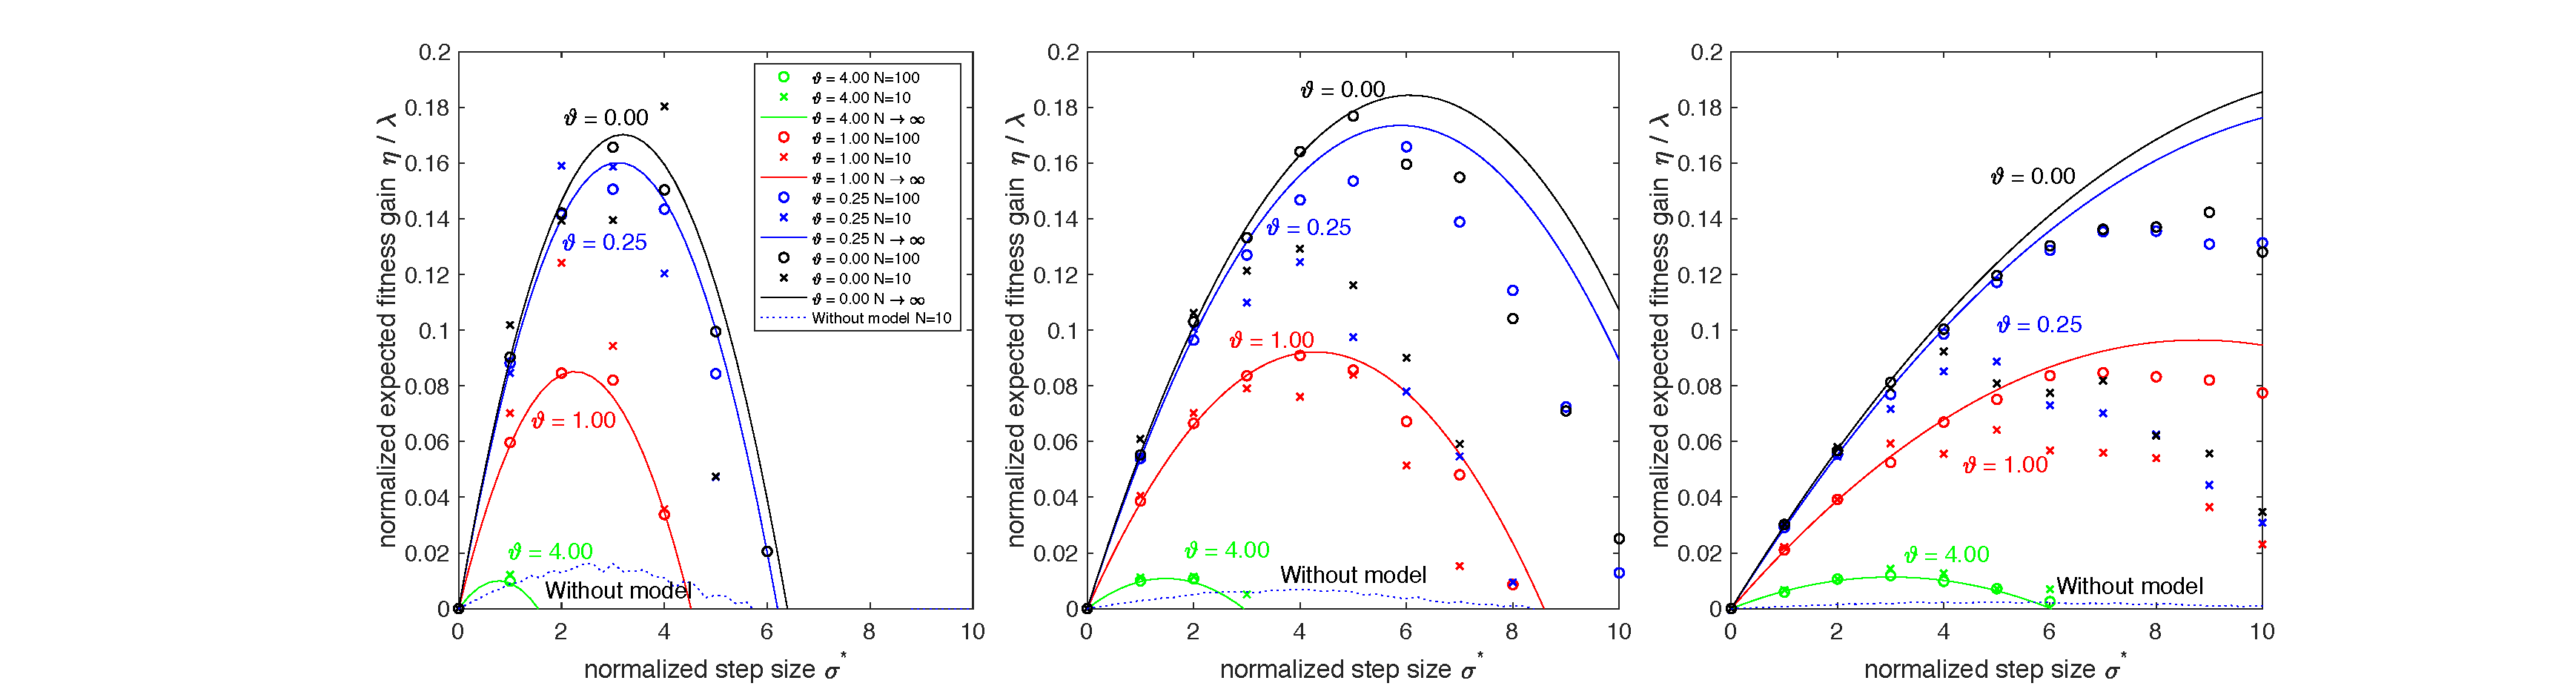
\includegraphics[height=2.7in, width=7.1in]{expectedFitGain_v1}
\caption{The figures from left to right shows the expected signle step behaviour of the surrogate model assisted $(\mu/\mu,\lambda)$-ES with unbiased Gaussin distributed surrogate error with $\lambda=10,20,40$ respectively where $\mu = ceil(\lambda/4)$. The solid lines are the results obtained analytically when $n \rightarrow \infty$, while the dotted line below illustrates the corresponding performance ($n=10$) of the $(\mu/\mu,\lambda)$-ES without model assistance. The dots represents the experimental result for $n=10$ (croesses) and $n=100$ (circles).}
\end{figure*}
\end{center}

To understand the potential implications of using surrogate models in EAs with varying population size, in this section, we use a simple model that applis a surrogate on the population. Specifically, we propose an EA that, in each iteration, a population of new $\lambda$ candidate solutions are generated and then evaluated by the surrogate instead of true obejctive function calls and a selection based on the inaccurate surrogate estimate is done followed by a true objective function evaluation for the centroid of the selected referred to as the parent for next iteration. We assume that the inaccurate estimate of the surrogate model is a Gaussin random variable with mean equals the true objective function value of the candidate solution with some variance that describes the accuracy of the surrogate model. So, we can apply the technique of analyzing ESs's behaviours in the presence of Gaussian noise \cite{arnold2002noisy}. The analysis could be extend to biased surrogate modlels where the distribution mean is different from the exact objective function value\cite{DBLP:conf/ppsn/KayhaniA18}.....


Comparision based surrogate model 

% Formulation of problem
Consider the minimization of the quadratic sphere $f: \mathbb R^N \rightarrow \mathbb R$ with $f(x)=x^Tx$ where the surrogate model assisted $(\mu/\mu.\lambda)$-ES is applied. This section will use the surrogate model described above to replace the true objective function calls of candidate solutions in each iteration, inaccurate but at vanishing cost. We first consider a simple iteration of the strategy. In each iteration, a population size of $\lambda$ new candidate solutions $y_i \in \mathbb{R}^N,i = 1,...,\lambda $ are generated from $\mu$ parents $x_i \in \mathbb{R}^N, i=1,...,\mu$, where $\lambda>\mu$. The parental population with size $\mu$ are replaced by the best $\mu$ candidate solutions $y_{i;\lambda},i = 1,2,...,\mu$ evaluated by the surrogate model with fitness estimate $f_{\epsilon}(y_{i;\lambda}) \leq f_{\epsilon}(y_{j,\lambda}), 1 \leq i < j \leq \lambda$ at vanishing cost. For each of the $\lambda$ candidate solutions $y_i=x + \sigma z$ where the parent $x = \sum_{i=1}^n x_i/\mu$, the centroid of the parental population is obtained through intermediate recombination, $z \in  \mathbb R^N$ is a standard normally distributed random vector, $\sigma > 0$ is the step size of the strategy that the adaptation is discussed in Section 4. The strategy uses the surrogate model to obtain a fitness estimate of the candidate solution $f_{\epsilon} (y_i), 1 \leq i \geq \lambda$ and by the assumption the estimate has mean $f(y_i)$ with some standard deviation $\sigma_\epsilon > 0$ (\textit{surroagte model error} also as \textit{fitness noise} \cite{1284729}). Better surrogate model results in smaller model error $\sigma_\epsilon$. For the $\lambda$ new candidate solutions $f_\epsilon (y_i) < f_\epsilon (y_j), 1 \leq i < j \leq \lambda$ indiccates the estimated objective function value of $y_i$ is superior to $y_j$ and therefore the best $\mu$ candidate solutions are selected,replacing the old parental population of size $\mu$ (used for offspring generation in next iteration), while the other inferior candidate solutions are discarded. Therefore, in each iteration only one objective function call is made in evaluating the fitness of the parent (centroid of parental population). The surrogate essentially does a pre-selection for $(\mu/\mu,\lambda)$-ES over candidate solutions, avoiding the unecessary objective function calls determined by the surroagte model.  

% The expected fitness gain over noise-to-signal ratio
Decomposition of $z$, first proposed by Rechenberg \cite{rechenberg1973evolutionsstrategie} can be used to study the expected step size of the strategy. We can decompose the vector $z$ as a vector sum $z = z_1 + z_2$, where $z_1$ is in the direction of the negative gradient of the objecive function $\nabla f(x)$, while $z_2$ orthogonal to $z_1$. We have $z_1$ standard normally distributed, while $\Vert z_2\Vert^2$ $\chi$-distributed with $N-1$ degree of freedom and $ \Vert z_2\Vert^2 /N \overset{N \rightarrow \infty }{=} 0$ (see reference theorem [$\color{red}{dirk's\ slides }$]). Denote $\delta = N (f(x) - f(y))/(2R^2)$ where $R = \Vert x \Vert$ is the distance to the optimal, we further introduce normalized step size $\sigma^* = N \sigma/R$ and $z_{\text{step}} = \sum_{i=1}^\mu z_{i;\lambda}$ (the averaged $z$ taken by the best $mu$ candidate solutions). The normalized fitness advantage of $y$ over $x$ follows
\begin{align}
\delta & = \frac{N}{2R^2} (x^Tx - (x+\sigma z_{\text{step}})^T (x+\sigma z_{\text{step}})) \nonumber\\
& = \frac{N}{2R^2} (-2 \sigma x^Tz_{\text{step}} - \sigma^2 \Vert z_{\text{step}}\Vert^2 ) \nonumber\\
& \overset{N \rightarrow \infty}{=} \sigma^* z_{\text{step},1} - \frac{{\sigma^*} ^2}{2},
\end{align}

 % $\color{red}{??? 1 \text{ or }\mu ???}$ assuming $\mu \ll N$
where $z_{\text{step},1} $, the component of $z_{\text{step}}$ pointing to the negative graident of $f(x)$, is normally distributed and $\overset{ N \rightarrow \infty}{=}$ denotes the convergence of the distribution $\Vert z_{\text{step} } \Vert^N/N = 1$. We further indtroudce $\sigma_\epsilon^* = N \sigma_\epsilon / (2R^2)$, the normalized surrogate model error (also referred to as the normalized fitness noise in Noise Sphere from Arnold and Beyer \cite{1284729}). The estimate of true objective function value of $y_i$ is $f_\epsilon (y_i) = f(y_i) + \sigma_\epsilon z_\epsilon, z_\epsilon \in \mathbb{R}$ is standard normally distributed.

The actual normalized fitness advantage of $y$ using the surrogate model is 
\begin{align}
\delta_\epsilon = \delta+\sigma_\epsilon^* z_\epsilon 
\end{align}

The expected value of the normalized change in objective function value  
\begin{align}
\Delta &= -\frac{N}{2} E \left [  \log f(y) - \log {f(x)} \right ] \nonumber\\
 &= -\frac{N}{2} E \left [  \log \frac{f(x^{t+1})}{f(x^{t})} \right ], 
\end{align}

where $y^{t}$ is the centroid of parental population in timestamp $t$, the equation is normalized in terms of dimensionality.

Since the fitness of $\lambda$ offspring generated are evaluated by the surrogate model with vanishing cost. The objective function evaluation per iteration is 1 instead of $\lambda$ (for $(\mu/\mu,\lambda)$-ES), therefore the normalized progress rate when dimensionality $N \rightarrow \infty$, by substituting $\lambda$ with 1 in equation (7) from \cite{ARNOLD2001127} is 
\begin{align}\label{eta}
\eta = \frac{1}{1}E[ \Delta] = \frac{\sigma^* c_{\mu / \mu, \lambda}}{\sqrt {1+ \vartheta^2}} - \frac{(\sigma^*)^2}{2 \mu},
\end{align}
where $\vartheta = \sigma_\epsilon^*/\sigma^*$ is the noise-to-signal ratio, defined to measure the quality of surrogate model relative to the algorithm's step size, $c_{\mu/\mu,\lambda}$ is the $(\mu/\mu,\lambda)$-progess coefficient derived by Arnold and Beyer \cite{Arnold:2000:EMS:645825.669117} that follows
% $\color{red}{paper\ missing}$
\begin{align}\label{c_mu_mu_lambda}
c_{\mu/\mu,\lambda}  = \frac{\lambda-\mu}{2 \pi} \begin{pmatrix} \lambda \\ \mu \end{pmatrix} \int_{-\infty}^{\infty} e^{-x^2}   \left [ \Phi(x)\right]^{\lambda-\mu-1}  \left[ 1- \Phi (x) \right]^{\mu-1}  \text{d} x,
\end{align}
where $\Phi^{-1}$ is the inverse function of $\Phi$, the normal cumulative distribution function. The integral can be solve numerically.  

To obtain the opt. expected fitness gain $\eta_{opt}$ and its coresponding opt. normalized step size $\sigma^*_{opt}$, we take derivative of equation (\ref{eta}) over $\sigma^*$ and get the following 
\begin{align}\label{opt}
\eta_{opt} &= \frac{\sigma^*_{opt} c_{\mu \ \mu, \lambda}}{\sqrt {1+ \vartheta^2}} - \frac{(\sigma^*_{opt})^2}{2 \mu} \\
\sigma^*_{opt} &= \frac{ \mu c_{\mu \ \mu, \lambda}}{\sqrt {1+ \vartheta^2}}
\end{align}

The expected fitness gian is normalized in terms of the population size $\lambda$ for easy comparision. The normalzied fitness gain against the normalized step size for $(\mu/\mu,\lambda)$-ES with population size $\lambda=10,20,40$ corresponding $\mu=3,5,10$ are ploted in Figure 1 from left to right respectively. The line shows the result obtained from Eqs. (\ref{eta}) (\ref{c_mu_mu_lambda}). The dots represent the experimental result for unbiased Gaussin surroagte error for $n \in \{10,100 \}$ obtained by averaging 100 runs. The result obtained for $n \rightarrow \infty$ are considered to be cases with a large normalized step size with very small noise to signal ratio. 

It can be inferred from Figure 1, for a fixed population size, the expected fitness gain decreases with an increasing noise-to-signal-ratio. When $\vartheta \rightarrow \infty$, the surrogate model becomes useless and the strategy becomes a random search. 
% random -- the strategy becomes a $\color{red}{\text{random search?? no selection but still take average is there a name for this? }} $. The expected fitness gain increases proportionally with an increasing population size and the maximal 

Compared the result obtained by the surrogate assisted (1+1)-ES (Fig 1. \cite{DBLP:conf/ppsn/KayhaniA18}), there is indeed a 

there is a significant increase in expected fitness gain as the population size $\lambda$ increases, the 

% The expected fitness gian against the normalized step size for (1+1)-ES is ploted in Fig. 1 (\cite{DBLP:conf/ppsn/KayhaniA18} and $(\mu/\mu,\lambda)$-ES with population size $\lambda=10,20,40$ in Fig. 2, Fig. 3 and Fig. 4 respectively. The line shows the result obtained from Eqs. (4),(5),(6) for (1+1)-ES from Arash and Dirk \cite{DBLP:conf/ppsn/KayhaniA18} and (\ref{eq:eta}) (\ref{eq:c_mu_mu_lambda}) for $(\mu/\mu,\lambda)$-ES. The dots represent the experimental result for unbiased Gaussin surroagte error for $n \in \{10,100 \}$ obtained by averaging 100 runs. The result obtained for $n \rightarrow \infty$ are considered to be cases with a large normalized step size with very small noise to signal ratio. 



\begin{center}
\begin{figure*}
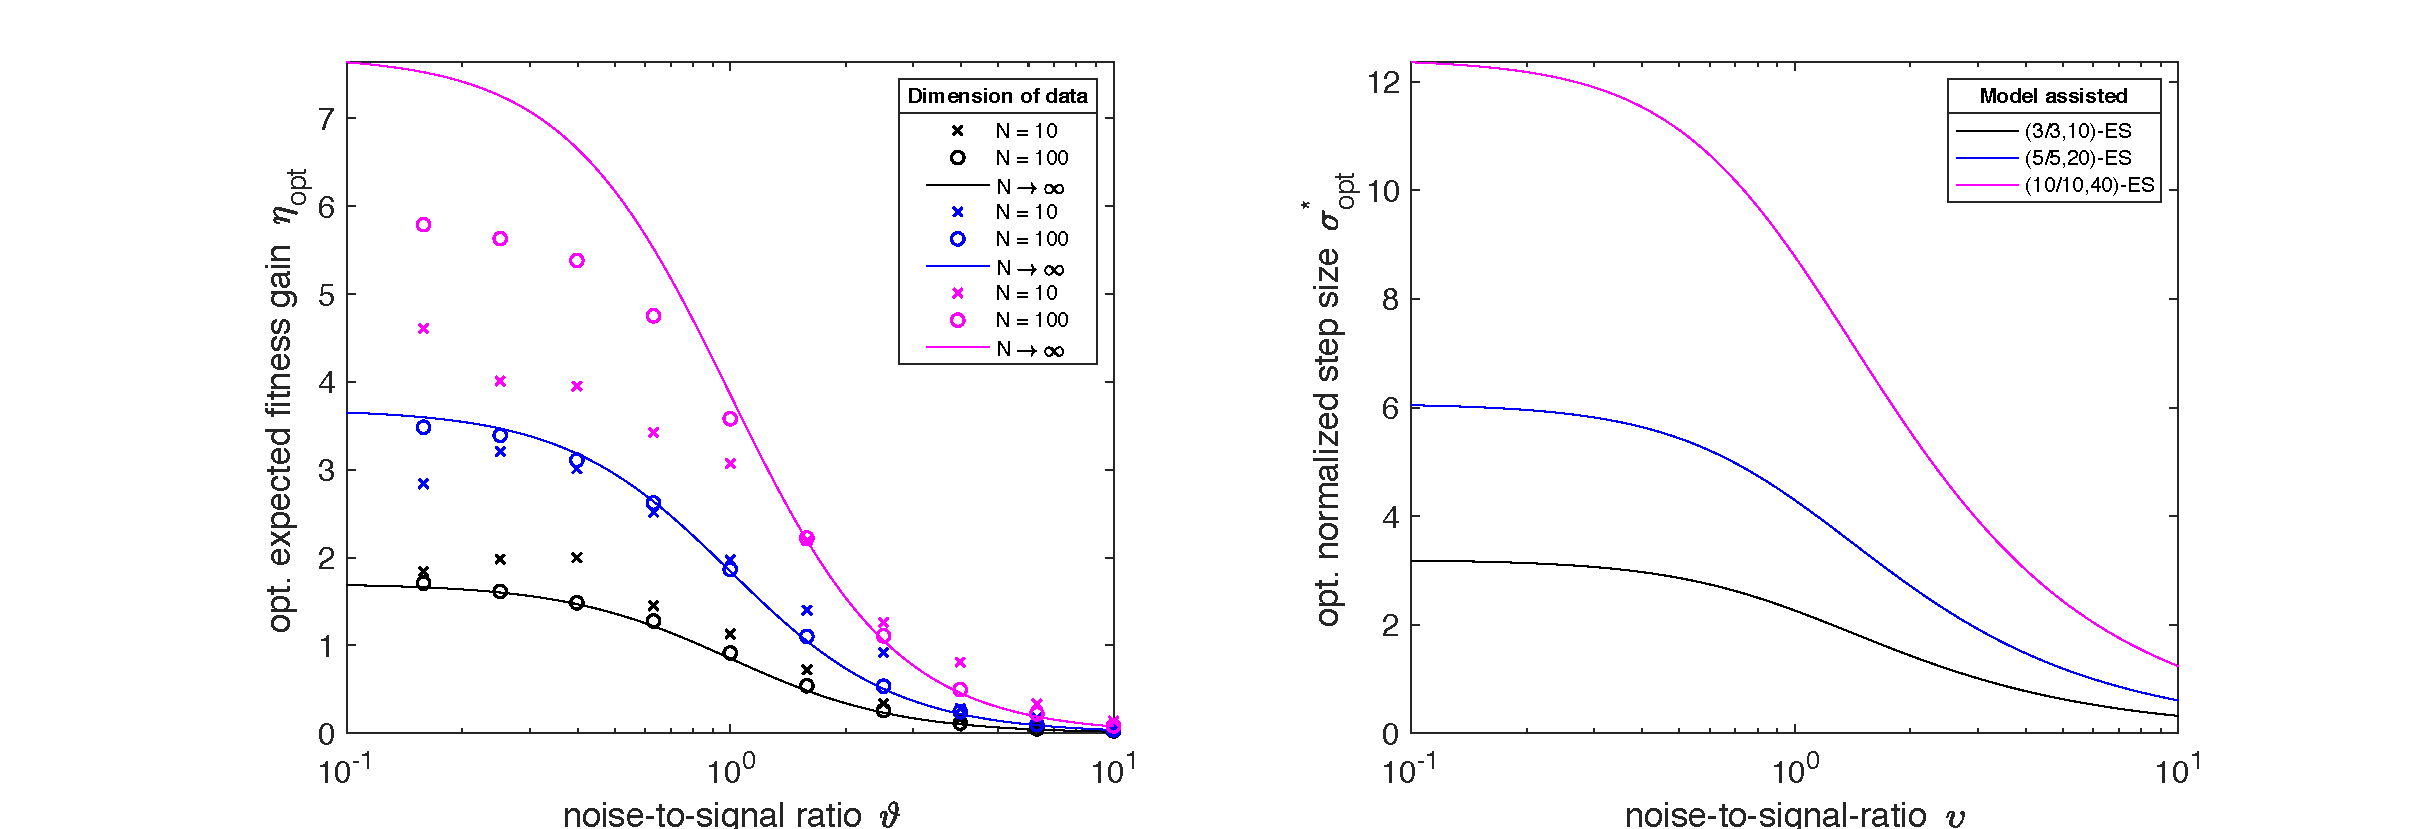
\includegraphics[height=2.2in, width=4.8in]{opt_stepSize_fitGain_v1}
\caption{Opt. expected fitness gain and corsponding opt. normalized step size of the surrogate model assisted $(\mu/\mu,\lambda)$-ES plotted against the noise-to-signal ratio. The line and dots with colour black, blue green represent $(3/3,10)$-ES, $(3/3,10)$-ES, $(3/3,10)$-ES The solid line representa the results obtained analytically when $n\rightarrow \infty$. }
\end{figure*}
\end{center}

% $\color{red}{(log\ sclae\ size)}$


% $\color{red}{graph- subplot(1,3)\ seems\ better?}$

% $$g(x,y,\sigma_\epsilon^*, \sigma^*)= 1/ \sqrt{2 \pi} e^{-y^2/2} p_{\alpha|z1}(x|y) \delta(x, y)$$

% The expected fitness gain relative to normalized step size is plotted in figure 2. The dots show the corresponding values observed in experiments with unbiased Gaussian surrogate error for $n \in \{10, 100\}$ obtained by averaging 40 runs. We tried to compute the expected fitness gain ($n \rightarrow \infty$) over the normalized step size analytically, but feailed because the function to integrate does not seem to converge over $y$. We experimented with different values of $\sigma_\epsilon^*$ and $\theta$ for $g(x,y,\sigma_\epsilon^*, \sigma^*)$ but the value obtained is a negative constant along the y-axes when $y$ exceeds a certain value for a range of $x$. An example of the plot for $g(x,y,\sigma_\epsilon^*, \sigma^*)$ over $x$ and $y$ with $\sigma_\epsilon^*=1$ and $\sigma^*=1$ is shwon in Fig.3 where two half-cylinder-shape along y-axes can be observed. $n \rightarrow \infty$ can be intepreted as a large step size with small noise-to-signal ratio.  



% It can be seen from Fig.2 that for a small noise-to-signal ratio, the evaluation rate increases with an increasing step size. While for a large noise-to-signal ratio, evaluation rate decreases with an increasing step size. The strategy makes progress one out of two steps for very small step size. The strategy becomes more "wise" in generating offsprings with a large step size and a relative small noise-to-signal ratio in a sense that the candidate solution optimized in this iteration is more close to the true lowest point of the quadratic model with a relative large space for candidate generation. In the case of zero noise-to-signal ratio, the candidate solution is deemed superior to its parent by choosing the best candidate solution in the direction sampled. 

% The expected fitness gain decreases as the step size increases (observed in Fig. 2 $\theta = 4$ green dots) which is contrary to the case where $\theta = 0.25$ and $\theta = 1$. One intepretation is that the strategy samples one direction in each iteration and the candidate solution is optimized in that direction using a quadratic model. The fitness gain of the candidate solution largely depends on the direction sampled and the accurancy of the estimation for the points fitting the quadratic model. The noise-to-signal ratio $\theta$ controls the precision of the optimal candidate solution estimtaed in the quadratic model relative to step size. A large $\theta$ means the estimation of the optimal candidate solution in the direction sampled is less accurate and therefore the evaluation rate decreases as the step size increases (the increasing step size also adds inaccurancy to the estimation of the optimal candidate solution).  

% The direction sampled also affects the model performance. We would like to optimize the candidate solution in a direction with a potentially large fitness gain. But random sampling makes the process uncertain and according to experimental results, chances are that we do not sample a good direction in most cases i.e. the imporvement for the parent is limitted. So that a selection mechanism for the (direction of) candidate solutions in each iteration should be further considered. One possible approach is to consider the difference (distance) of the candidate solution before and after optimization using the quadratic model. Or we could possibly try unit vectors in each dimension, optimize using the quadratic model and choose the direction with the largest absolute $-2a/b$ (surrogate step size) in the optimization using the quadratic model.

% % \begin{figure}
% % \includegraphics[height=2in, width=3in]{IntXY}
% % \caption{The function to integrate over $x$ and $y$ with $\sigma_\epsilon^*=1$ and $\sigma^*=1$ i.e. $g(x,y,1,1)$ over $x$ and $y$. Notice the two half cylinders along y-axes where the function value for each $x$ is a negative constant. }
% % \end{figure}




% For a fixd dimensionality $N$ the normalized progress rate \cite{ARNOLD2002629} is 


% $$
% \eta \approx \frac{c_{\mu/\mu,\lambda} \sigma^* (1+{\sigma^*}^2 /2\mu N)}{\sqrt{ 1+{\sigma^*}^2 /2\mu N) } \sqrt{ 1+ \vartheta^2 +{\sigma^*}^2 /2N }} - N \left [ \sqrt{1+ \frac{ {\sigma^*}^2 }{\mu N} - 1} \right ] 
% $$




\section{Step size adaptation}

\subsection{Cummulative step size adaptation}

Even though the analysis in Section 3 suggests potential better performance for the surrogate-assisted $(\mu/\mu,\lambda)$-ES. There is no gaurantee the step size of the strategy can be properly adapted and further the analysis is very inaccurate in terms of finite dimension. In this section we experiemnt the surroagted model assisted $((\mu/\mu,\lambda)+(\mu/\mu,\lambda))$-ES using the cumulative step size adaptation (CSA)\cite{Ostermeier:1994:DAS:1326675.1326679}, commonly used in $(\mu/\mu,\lambda)$-ES and exploit the potential insight that it may offer. The strategy is evaluated by using a Gaussian Process based surrogate model replacing the simple model that simulates the surrogate behaviour in Section 3. Several test functions are used for testing the strategy.

% $\color{red}{(normalized\ step\ size)}$



% $\color{red}{table(test\ functions)}$

Table for median of test results for surrogate model assisted $(\mu/\mu,\lambda)$-ES using CSA


% $\color{red}{histgram\ obejective\ function\ evaluations\ AND\ plot\ model\ error\ AND\ normalized\ step\ size)}$

Figure histogram for objective function evaluations and relative surrogate model error. 

% $\color{red}{histgram\ success\ rate\ AND\ normalized\ convergence\ rate(3\ sphere\ functions) }$

Figure for success rate for surroagte assisted $(\mu/\mu,\lambda)$-ES with $\lambda = 10,20,40$





\begin{table*} 
\caption{Median test results.}
\begin{tabular}{ l *{5}{D{.}{.}{4}} }
\toprule
\textbf{} & \multicolumn{5}{c}{\textbf{Median number of objective function calls (with model assistance) }} \\
\cmidrule(lr){2-6}
\textbf{Test functions} & \multicolumn{1}{c}{$(1+1)$-ES} & \multicolumn{1}{c}{$(3/3,10)$-ES} & \multicolumn{1}{c}{$(5/5,20)$-ES} & \multicolumn{1}{c}{$(10/10,40)$-ES}  \\
\midrule
\texttt{linear sphere} &503 &4.65\% &9.84\% &19.17\%      \\
\texttt{quadratic sphere} &214 &8.39\% &18.31\%  &28.09\% \\ 
\texttt{cubic sphere} &198 &8.64\% &14.51\% &25.83\%      \\ 
\texttt{Schwefel\' s function} &1503 &18.28\% &31.58\% &64.43\%\\ 
\texttt{quartic function} &1236 &7.37\% &15.55\% &32.48\%    \\ 
        \bottomrule             
\end{tabular}
\label{Tab:Test_result}
\end{table*}

% \renewcommand{\arraystretch}{1.5} %控制行高
% \begin{table}[tp]
 
%   \centering
%   \fontsize{6.5}{8}\selectfont
%   \begin{threeparttable}
%   \caption{Demographic Prediction performance comparison by three evaluation metrics.}
%   \label{tab:performance_comparison}
%     \begin{tabular}{ccccccc}
%     \toprule
%     \multirow{2}{*}{Methods}&
%     \multicolumn{1}{c}{median number of objective function calls (with model assistenace)}\cr
%     \cmidrule(lr){2-2} \cmidrule(lr){3-5}
%     &(1+1)-ES with model&$(3/3,10)-ES$&$(5/5,20)-ES$&$(10/10,40)-ES$\cr
%     \midrule
%     linear sphere&503&0.7388&0.7301&0.6371\cr
%     quadratic sphere&214&0.7385&0.7323&0.6363\cr
%     cubic sphere&198&0.7222&0.7311&0.6243\cr
%     Schwefel’s function&1503&0.7716&0.7699\cr
%     quartic function&1236&0.7317&0.7343\cr
%     \bottomrule
%     \end{tabular}
%     \end{threeparttable}
% \end{table}



% \begin{algorithmic}
% \STATE $c \rightarrow  \frac{\mu +2}{n+\mu+5}$
% \STATE $d \rightarrow 1 + 2 \text{max}(0, \sqrt{\frac{\mu - 1}{n+1} } - 1 ) $
% \STATE $p \rightarrow 0$
% \STATE $D \rightarrow 0.68$

% \WHILE{not terminate()} 
% 	\FOR{$i=1,2,...,\lambda$}
% 		\STATE Generate standard normally distributed $z_i \in \mathbb{R}^N $
% 		\STATE $y_i \rightarrow x + \sigma z_i$
% 		\STATE Evaluate $y_i$ using the surrogate model, yieding $\hat{f}(y_i)$
% 	\ENDFOR
% 	\STATE $z = \frac{1}{\mu} \sum_{i=1}^{\mu} z_{i;\lambda}$
% 	\STATE $y = x + \sigma x$
% 	\STATE Evaluate $y$ using true objective function, yieding $f(y)$
% 	\STATE Update surrogate modle 
% 	\IF{$f(x) < f(y)$ (Emergency)}
% 		\STATE $\sigma \rightarrow \sigma D$
% 	\ELSE[]
% 		\STATE $s \rightarrow (1-c)s + \sqrt{ c(2-c) \mu z}$
% 		\STATE $\sigma \rightarrow \sigma \text{exp} \left (\frac{c}{d} \left ( \frac{\| p\|}{ E\| \mathscr{N}(0,I)\|} -1 \right ) \right )$
% 	\ENDIF

% \ENDWHILE
%    \STATE $S \leftarrow 0$

% \end{algorithmic}
% $\sigma \leftarrow \sigma \text{exp}  (\frac{c}{d}  ( \frac{\| p\|}{ E\| \mathscr{N} (0,I) \|} -1 )  )$

\begin{algorithm}
\caption{A Surrogate Assisted $(\mu/\mu,\lambda)$-ES}
\label{alg}
\begin{algorithmic}[1]
\STATE $c \leftarrow  \frac{\mu +2}{n+\mu+5}$ 
\STATE $d \leftarrow 1 + 2 \text{max}(0, \sqrt{\frac{\mu - 1}{n+1} } - 1 ) $
\STATE $p \leftarrow 0$

\WHILE{not terminate()} 
	\FOR{$i=1,2,...,\lambda$}
		\STATE Generate standard normally distributed $z_i \in \mathbb{R}^N $
		\STATE $y_i \leftarrow x + \sigma z_i$
		\STATE Evaluate $y_i$ using the surrogate model, yieding $f_{\epsilon}(y_i)$
	\ENDFOR
	\STATE $z = \frac{1}{\mu} \sum_{i=1}^{\mu} z_{i;\lambda}$
	\STATE $y = x + \sigma x$
	\STATE Evaluate $y$ using true objective function, yieding $f(y)$
	\STATE Update surrogate modle 
	\STATE $s \leftarrow (1-c)s + \sqrt{ c(2-c) \mu z}$
	\STATE $\sigma \leftarrow \sigma \times \text{exp} \left(\frac{c}{d} \frac{\left\lVert X \right\rVert} { E \left\lVert N(0,I) \right\rVert} -1 \right )$
		

\ENDWHILE

\end{algorithmic}
\end{algorithm}




\subsection{Alternative}

From Figure x, the success rate for all test functions are approxiamtely 0.48, the strategy makes a bad step every other step. It comes natural to ask, how much we are to benefit if we can avoid or simplily not take those bad steps.  


Recent papers in surroagte model assisted ES consider (1+1)-ES, the step size of the stratgey is successfully adapted using the 1/5-rule []. Then we probbaly can apply a similar criteria when encounter a bad step size. 

Propose step size adaptation in terms of emergency.

\begin{algorithm}
\caption{Cummulative Step Size Adaptation with Emergency}
\label{alg}
\begin{algorithmic}[1]
\STATE $c \leftarrow  \frac{\mu +2}{n+\mu+5}$ 
\STATE $d \leftarrow 1 + 2 \text{max}(0, \sqrt{\frac{\mu - 1}{n+1} } - 1 ) $
\STATE $p \leftarrow 0$
\STATE $D \leftarrow 0.68$

\WHILE{not terminate()} 
	\FOR{$i=1,2,...,\lambda$}
		\STATE Generate standard normally distributed $z_i \in \mathbb{R}^N $
		\STATE $y_i \leftarrow x + \sigma z_i$
		\STATE Evaluate $y_i$ using the surrogate model, yieding $\hat{f}(y_i)$
	\ENDFOR
	\STATE $z = \frac{1}{\mu} \sum_{i=1}^{\mu} z_{i;\lambda}$
	\STATE $y = x + \sigma x$
	\STATE Evaluate $y$ using true objective function, yieding $f(y)$
	\STATE Update surrogate modle 
	\IF{$f(x) < f(y)$ (Emergency)}
		\STATE $\sigma \leftarrow \sigma D$
		
	\ELSE
		\STATE $s \leftarrow (1-c)s + \sqrt{ c(2-c) \mu z}$
		\STATE $\sigma \leftarrow \sigma \times \text{exp} \left(\frac{c}{d} \frac{\left\lVert X \right\rVert} { E \left\lVert N(0,I) \right\rVert} -1 \right )$
		
	\ENDIF


\ENDWHILE
\end{algorithmic}
\end{algorithm}

$\color{red}{table(test\ functions)}$
Table for median of test results for surrogate model assisted $(\mu/\mu,\lambda)$-ES using CSA with emergency


Figure for success rate for surroagte assisted $(\mu/\mu,\lambda)$-ES with $\lambda = 10,20,40$



\section{Conclusions}
In this paper, We proposed a local surrogate-assisted $(\mu/\mu,\lambda)+(\mu/\mu,\lambda)$-ES. The strategy uses a lcoal surrogate model to optimize the candidate solution obtained in each iteration. The performance is analyzed by adding different levels of Gaussian distributed noise and applying the strategy to sphere functions. 

% For future work, we will work on a selection mechanism for candidate solutions deciding what candidate solutions to choose based on the fitness gain it may bring. Further, a step size adaptation mechanism for the surrogate model assisted (1 + 1)-ES should be considered. 


%\end{document}  % This is where a 'short' article might terminate




% \appendix
% %Appendix A
% \section{Headings in Appendices}
% The rules about hierarchical headings discussed above for
% the body of the article are different in the appendices.
% In the \textbf{appendix} environment, the command
% \textbf{section} is used to
% indicate the start of each Appendix, with alphabetic order
% designation (i.e., the first is A, the second B, etc.) and
% a title (if you include one).  So, if you need
% hierarchical structure
% \textit{within} an Appendix, start with \textbf{subsection} as the
% highest level. Here is an outline of the body of this
% document in Appendix-appropriate form:
% \subsection{Introduction}
% \subsection{The Body of the Paper}
% \subsubsection{Type Changes and  Special Characters}
% \subsubsection{Math Equations}
% \paragraph{Inline (In-text) Equations}
% \paragraph{Display Equations}
% \subsubsection{Citations}
% \subsubsection{Tables}
% \subsubsection{Figures}
% \subsubsection{Theorem-like Constructs}
% \subsubsection*{A Caveat for the \TeX\ Expert}
% \subsection{Conclusions}
% \subsection{References}
% Generated by bibtex from your \texttt{.bib} file.  Run latex,
% then bibtex, then latex twice (to resolve references)
% to create the \texttt{.bbl} file.  Insert that \texttt{.bbl}
% file into the \texttt{.tex} source file and comment out
% the command \texttt{{\char'134}thebibliography}.
% % This next section command marks the start of
% % Appendix B, and does not continue the present hierarchy
% \section{More Help for the Hardy}

% Of course, reading the source code is always useful.  The file
% \path{acmart.pdf} contains both the user guide and the commented
% code.

% \begin{acks}
%   The authors would like to thank Dr. Dirk V. Arnold for providing the
%   MATLAB code of the \textit{BEPS} method.

%   The authors would also like to thank the anonymous referees for
%   their valuable comments and helpful suggestions. The work is
%   supported by the \grantsponsor{GS501100001809}{National Natural
%     Science Foundation of
%     China}{http://dx.doi.org/10.13039/501100001809} under Grant
%   No.:~\grantnum{GS501100001809}{61273304}
%   and~\grantnum[http://www.nnsf.cn/youngscientists]{GS501100001809}{Young
%     Scientists' Support Program}.

% \end{acks}


